\documentclass[10pt]{article}
\usepackage{pgf,tikz}
\usetikzlibrary{arrows}
\pagestyle{empty}
\begin{document}
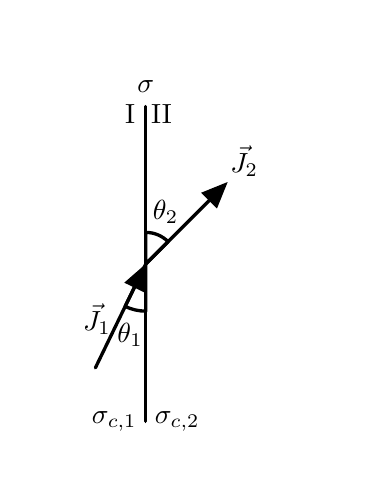
\begin{tikzpicture}[line cap=round,line join=round,>=triangle 45,x=1.0cm,y=1.0cm]
\clip(-1.5,-2.5) rectangle (2.5,3);
\draw [shift={(0,0)},line width=1.2pt] (0,0) -- (-115.96:0.6) arc (-115.96:-90:0.6) -- cycle;
\draw [shift={(0,0)},line width=1.2pt] (0,0) -- (45:0.4) arc (45:90:0.4) -- cycle;
\draw [line width=1.2pt] (0,2)-- (0,-2);
\draw [->,line width=1.2pt] (0,0) -- (1.04,1.04);
\draw [->,line width=1.2pt] (-0.64,-1.32) -- (0,0);
\draw (0,2.25) node[anchor=center] {$\sigma$};
\draw (-0.2,1.9) node[anchor=center] {I};
\draw (0.2,1.9) node[anchor=center] {II};
\draw (0.4,-2) node[anchor=center] {$\sigma_{c,2}$};
\draw (-0.4,-2) node[anchor=center] {$\sigma_{c,1}$};
\draw[color=black] (1.25,1.3) node {$\vec J_2$};
\draw[color=black] (-0.62,-0.7) node {$\vec J_1$};
\draw[color=black] (-0.2,-0.9) node {$\theta_1$};
\draw[color=black] (0.25,0.66) node {$\theta_2$};
\end{tikzpicture}
\end{document}
